\section{No elementary closed form for the conjugacy when \texorpdfstring{$r\in(0,1)$}{r in (0,1)}}
\label{a:sec:ncf-main}

The obstruction rests on four short steps.  First, every elementary function is
differentially algebraic.  Second, differential algebraicity is preserved under
local compositional inversion.  Third, the Becker--Bergweiler classification
allows a differentially algebraic solution of Schr\"oder's equation for a rational
map of degree at least two only when the underlying fixed point is repelling.
Finally, for $r\in(0,1)$ the fixed point $0$ of $f_r$ is attracting.  It follows
that $\psi_r$ is hypertranscendental at every subcritical parameter, with no
exceptional case inside the attracting window.  The theorem has a strict boundary,
however: it does not by itself determine the arithmetic status of an individual
number $A(p_0)$ or the differential algebraicity of the map $p\mapsto A(p)$.  The
second half of the section separates these questions before presenting the
available numerical evidence.

\subsection{Differential algebraicity, hypertranscendence, elementarity}

\begin{definition}[differentially algebraic; hypertranscendental]
\label{a:def:da}
A function $g$, holomorphic on a domain (or a formal power series), is \emph{differentially algebraic over $\mathbb{C}(z)$} if there exists a non-zero polynomial $P$ in $n+2$ variables, for some $n\ge0$, with
\[
P\bigl(z,\,g(z),\,g'(z),\,\dots,\,g^{(n)}(z)\bigr)\equiv 0 .
\]
Otherwise $g$ is \emph{differentially transcendental}, or \emph{hypertranscendental}.
\end{definition}

Two closure properties make this the appropriate notion here.

\begin{lemma}[elementary $\Rightarrow$ differentially algebraic]
\label{a:lem:elem-da}
Every elementary function in the Liouville sense --- any function reachable from $\mathbb{C}(z)$ by a finite tower of algebraic operations, exponentials and logarithms --- is differentially algebraic. Consequently a hypertranscendental function is not elementary.
\end{lemma}

\begin{proof}[Proof sketch]
Each storey of a Liouvillian tower preserves differential algebraicity.  Algebraic
extensions do so by elimination; if $g$ is differentially algebraic, then the
first-order defining relations for $e^g$ and $\log g$ combine with the equation for
$g$; and the class is closed under field operations and composition.  These
closure properties are classical; see Rubel's survey \cite{Rubel1989}.
\end{proof}

\begin{lemma}[closure under compositional inversion]
\label{a:lem:inv-da}
Let $g$ be holomorphic near $0$ with $g(0)=0$ and $g'(0)\neq0$, and let $g^{-1}$ denote its local compositional inverse. Then $g$ is differentially algebraic over $\mathbb{C}(z)$ if and only if $g^{-1}$ is (Moore \cite{Moore1896}; see also Boshernitzan--Rubel \cite{BoshernitzanRubel1986}).
\end{lemma}

The inversion lemma is needed because the literature uses two opposite but
equivalent conventions for Schr\"oder's equation.  Here $\psi_r$ is the
\emph{linearising coordinate}, satisfying
$\psi_r(f_r(z))=r\,\psi_r(z)$.  Becker and Bergweiler, following Ritt, classify
the inverse \emph{linearising parametrisation} $\varphi_r=\psi_r^{-1}$, which
satisfies
\begin{equation}
\label{a:eq:schroder-param}
\varphi_r(r\,t)=f_r\bigl(\varphi_r(t)\bigr),
\qquad
\varphi_r(0)=0,\quad \varphi_r'(0)=1 .
\end{equation}
By \Cref{a:lem:inv-da}, the two conventions have the same differential-algebraic
status.

\subsection{The Becker--Bergweiler theorem, stated precisely}

The required result is the 1995 classification of differentially algebraic
Schr\"oder functions \cite{Becker1995}, quoted here in the form given in Fernandes'
survey of the Schr\"oder, B\"ottcher and Abel equations
\cite[Thm~3.1]{Fernandes2021}.

\begin{theorem}[Becker--Bergweiler \cite{Becker1995}; as restated in {\cite[Thm~3.1]{Fernandes2021}}]
\label{a:thm:BB-main}
Let $R$ be a rational map of degree at least two with $R(0)=0$ and multiplier $s=R'(0)$, where $s\neq0$ and $s$ is not a root of unity (for $|s|=1$ the Schr\"oder function is understood as a formal series). Let $\varphi$, normalised by $\varphi(0)=0$ and $\varphi'(0)=1$, solve $\varphi(st)=R(\varphi(t))$. If $\varphi$ is differentially algebraic over $\mathbb{C}(t)$, then:
\begin{enumerate}[label=\textup{(\roman*)}]
\item the fixed point $0$ is \emph{repelling}, $|s|>1$; and
\item $\varphi$ is a M\"obius transformation of one of
\[
\exp(\alpha t^{\rho}),
\qquad
\cos(\alpha t^{\rho}+\beta),
\qquad
\wp(\alpha t^{\rho}+\beta),\ \wp^{2},\ \wp^{3},\ \wp'(\alpha t^{\rho}+\beta),
\]
where $\wp$ is a Weierstrass function, $\rho\in\mathbb{Q}$ is such that the function concerned is meromorphic on $\mathbb{C}$, $\alpha\neq0$, and $\beta$ is a fraction of a period. Correspondingly $R$ is M\"obius-conjugate to $z^{\pm d}$, to $\pm T_d$ (Chebyshev), or to a Latt\`es map.
\end{enumerate}
\end{theorem}

\begin{remark}[lineage and independent corroboration]
\label{a:rem:lineage}
For $|s|>1$, the Poincar\'e-function case, the classification begins with Ritt's
1926 result \cite{Ritt1926}.  Becker and Bergweiler completed the picture for the
three classical functional equations, and the later account by Aschenbrenner and
Bergweiler \cite{AschenbrennerBergweiler2015} assigns the exceptional list
explicitly to the repelling case.  Di~Vizio and Fernandes
\cite{DiVizioFernandes2021} provide independent difference-Galois corroboration:
their Theorems~1.2 and~4.2 require only that $s$ be neither zero nor a root of unity,
with no assumption $|s|>1$, and show that a differentially algebraic solution of
$y(R(x))=s\,y(x)$ in the present $\psi$-convention must satisfy a first-order
equation of Ritt type, $(y')^{\rho}=B(x)y^{\,j}$.  The structural conclusion used
below therefore does not depend on a single formulation of the theorem.
\end{remark}

\subsection{Hypertranscendence throughout the subcritical window}

\begin{theorem}[no exceptional parameters in $(0,1)$]
\label{a:thm:main-ht}
For every $r\in(0,1)$, the Koenigs function $\psi_r$ of $f_r(z)=rz(1-z)$ at $0$ is hypertranscendental over $\mathbb{C}(z)$: it satisfies no algebraic differential equation. In particular, $\psi_r$ is not an elementary function.
\end{theorem}

\begin{proof}
Fix $r\in(0,1)$.  The degree-two rational map $f_r$ fixes $0$, where its
multiplier $s=f_r'(0)=r$ satisfies $0<s<1$; thus the hypotheses of
\Cref{a:thm:BB-main} hold at an attracting fixed point.  If $\psi_r$ were
differentially algebraic, its local inverse $\varphi_r=\psi_r^{-1}$ would be
differentially algebraic by \Cref{a:lem:inv-da} and would solve
\eqref{a:eq:schroder-param} with the stated normalisation.
\Cref{a:thm:BB-main}(i) would then force $|r|>1$, contradicting
$r\in(0,1)$.  Hence $\psi_r$ is hypertranscendental, and
\Cref{a:lem:elem-da} gives non-elementarity.
\end{proof}

\begin{remark}[the exceptional set inside the window is empty, not merely avoided]
\label{a:rem:empty}
The affine conjugacy $c(r)=(2r-r^{2})/4$ from \Cref{a:lem:affine} sends
$r\in(0,1)$ to $c\in(0,\tfrac14)$, thereby avoiding the exceptional quadratic
parameters $c=0$ and $c=-2$, reached at $r=2$ and at $r=4$ respectively (with
$c=-2$ also reached at $r=-2$).  This parameter-plane observation is correct but
not sufficient as a proof, because it does not by itself establish that the
exceptional list is complete within the window.  Part~(i) of
\Cref{a:thm:BB-main} removes that ambiguity: differentially algebraic Schr\"oder
functions occur only over repelling fixed points, so the attracting window contains
no candidates to enumerate.  Consistently, the elementary cases in
Appendix~\ref{a:app:integrable} have the repelling multipliers $2$ and $4$ and are
Poincar\'e-type linearisations, not solutions available for $r\in(0,1)$.
\end{remark}

\begin{figure}[H]
\centering
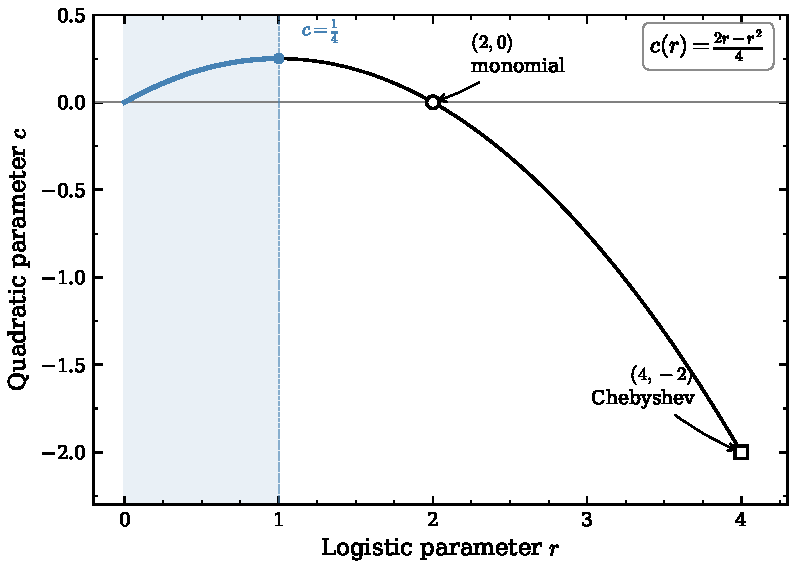
\includegraphics[width=0.72\textwidth]{figures/figure1_parameter_conjugacy.pdf}
\caption{Parameter correspondence $c(r)=(2r-r^2)/4$. The segment $r\in(0,1)$ maps to $c\in(0,\tfrac14)$, disjoint from the integrable values $c\in\{0,-2\}$. In the light of \Cref{a:rem:empty} this picture is a consistency check rather than the proof: the exceptional linearisations live over repelling fixed points, which the attracting window excludes outright.}
\label{a:fig:c-of-r}
\end{figure}

\begin{remark}[germ versus basin]
\label{a:rem:basin}
\Cref{a:thm:main-ht} concerns the analytic function $\psi_r$, whereas
$A(p)=2\Psi_r(\tfrac12)$ in \eqref{a:eq:A-koenigs} uses its extension to the real
basin of attraction.  For $p\geq\tfrac13$, the point $\tfrac12$ lies outside the
disc on which the Koenigs series is guaranteed to converge, whose radius is
$(1-r)/r$.  The functional equation nevertheless extends the germ by finitely many
pullbacks:
\[
\Psi_r(w)=r^{-N}\,\psi_r\bigl(f_r^{\circ N}(w)\bigr)
\quad\text{for $N$ large enough that $f_r^{\circ N}(w)$ enters the germ,}
\]
Any algebraic differential equation holding on a subdomain would persist under
this analytic continuation.  Hypertranscendence of the germ and of its basin
extension are therefore equivalent statements, and the identity
\eqref{a:eq:A-koenigs} is unaffected.
\end{remark}

\begin{figure}[H]
\centering
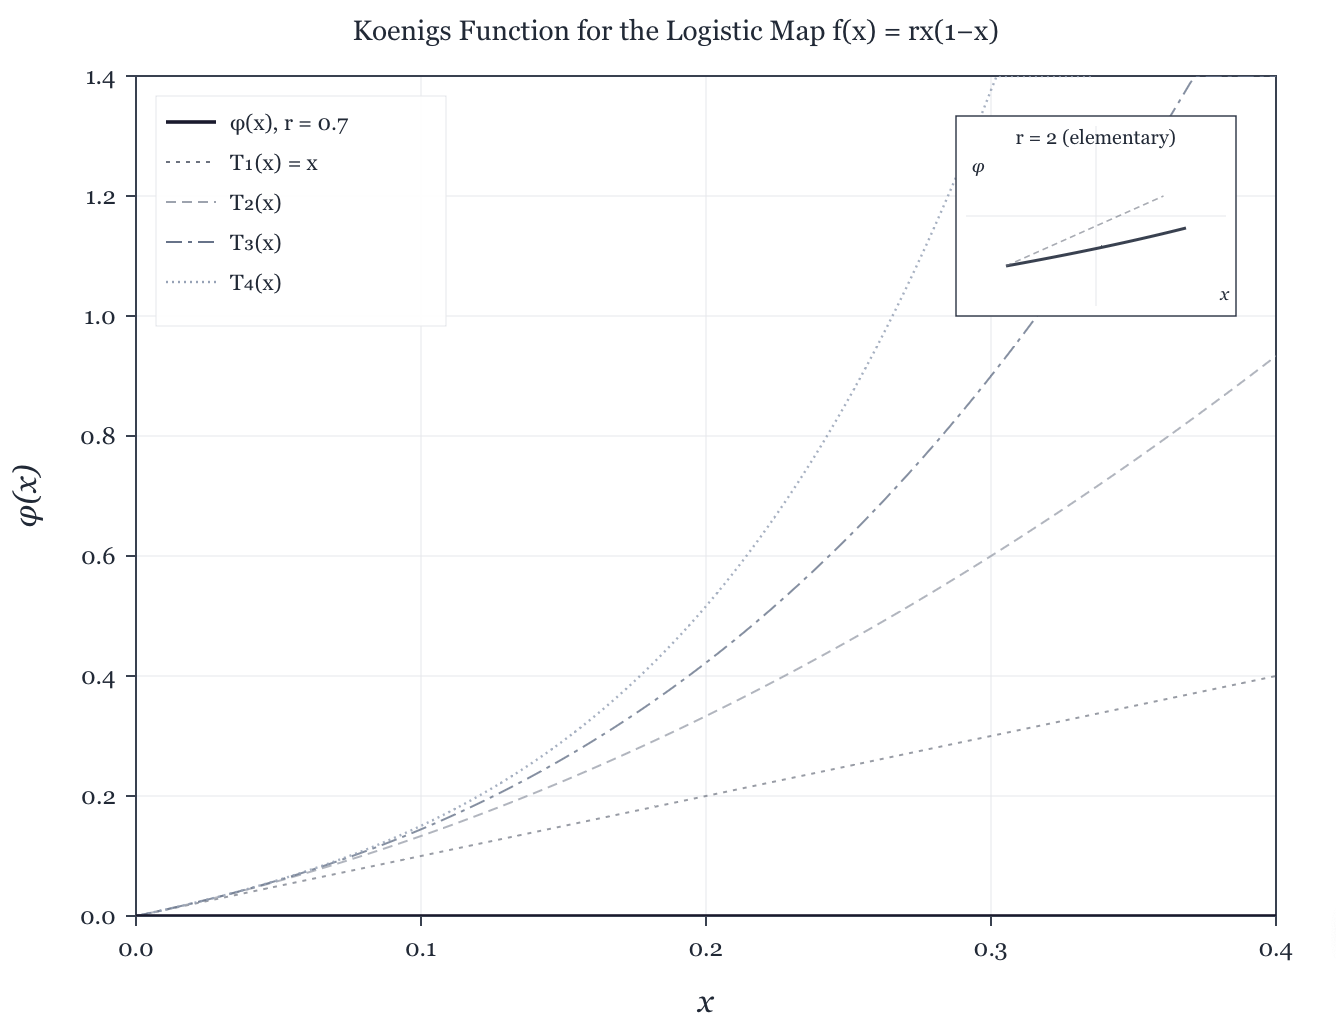
\includegraphics[width=0.72\textwidth]{figures/figure3_numerical_koenigs.png}
\caption{Numerical approximation of a Koenigs function for a logistic multiplier in $(0,1)$, with low-order Taylor polynomials near the origin. Elementary closed forms exist only for exceptional multipliers outside this range (Appendix~\ref{a:app:integrable}).}
\label{a:fig:koenigs-numeric}
\end{figure}

\subsection{What the theorem does and does not say about \texorpdfstring{$A(p)$}{A(p)}}
\label{a:subsec:scope}

The phrase ``closed form'' must be resolved before any claim about $A(p)$ is made.
At least four inequivalent readings occur here, and a result under one reading does
not transfer automatically to another:
\begin{enumerate}[label=\textup{(\Alph*)},leftmargin=*]
\item[\textbf{(V)}] the \emph{value} $A(p_0)$ is elementary or algebraic, for a fixed rational $p_0$;
\item[\textbf{(E)}] the \emph{map} $p\mapsto A(p)$ is an elementary function of $p$;
\item[\textbf{(D)}] the map is \emph{differentially algebraic in $p$}, i.e.\ satisfies some algebraic ODE in $p$;
\item[\textbf{(S)}] the map is expressible via standard special functions ($\Gamma$, $\zeta$, ${}_2F_1$, theta or $q$-series).
\end{enumerate}
At fixed $r$, \Cref{a:thm:main-ht} concerns the function
$z\mapsto\psi_r(z)$ and establishes exactly this: \emph{at no subcritical
parameter can evaluation of $A(p)$ be reduced to an algebraic differential
equation for the lineariser.}  The theorem does not by itself decide any of
(V), (E), (D) or (S).  Two gaps remain.

\paragraph{The value gap.}
A hypertranscendental function may take elementary, or even algebraic, values at
individual points.  H\"older's theorem makes $\Gamma$ hypertranscendental, for
example, while $\Gamma(\tfrac12)=\sqrt{\pi}$.  Nothing established above therefore
precludes $A(\tfrac14)$ from being algebraic.

There is a genuine values theorem nearby: Becker and Bergweiler proved in 1993
\cite{Becker1993} that the B\"ottcher conjugacy between two polynomials of the same
degree $d\geq2$ with algebraic coefficients, excluding maps linearly conjugate to
monomials or Chebyshev polynomials, is transcendental and takes transcendental
values at algebraic points.  Their proof uses Mahler's method; see Nishioka
\cite{Nishioka1996}.  That theorem does not transfer to the Koenigs value
$\psi_r(\tfrac12)$.  Formally, the Schr\"oder equation pairs an inner map of degree
two with the degree-one outer map given by multiplication by $r$, so the equal-
degree hypothesis fails.  Structurally, Mahler's method balances doubly exponential
analytic decay against comparable height growth.  Both exponents scale like
$d^{\,n}$ in the B\"ottcher setting, whereas the attracting Koenigs orbit
$w_n=f_r^{\circ n}(\tfrac12)$ decays only geometrically,
$|w_n|\sim Ar^n$, while the heights of the rational $w_n$ still grow doubly
exponentially, $h(w_n)\sim C2^{\,n}$.  The resulting inequalities therefore run in
the wrong direction at every $n$.  The obstruction lies in this degree structure,
not in the germ/basin distinction: the pullback in \Cref{a:rem:basin} moves the
evaluation point arbitrarily far into the germ at the cost of a rational factor.
Consequently,
\begin{center}
\emph{transcendence --- indeed, even irrationality --- of $A(p_0)$ is at present not proved\\ for a single rational $p_0\in(0,\tfrac12)$.}
\end{center}

\paragraph{The parameter gap.}
The map $p\mapsto A(p)$ lies outside \Cref{a:thm:main-ht}, so readings (E) and
(D) remain open and, to the best of our knowledge, unaddressed in the literature.
The most natural machinery is the parametrised differential Galois theory of
Hardouin and Singer \cite{HardouinSinger2008}, which detects differential
relations in auxiliary directions for linear difference equations such as
$\sigma\psi=r\psi$.  It does not apply directly here because $\partial_r$ fails to
commute with the substitution operator $\sigma\colon w\mapsto f_r(w)$, which itself
depends on $r$.  The near-critical asymptotics provide no alternative obstruction:
the logarithmic corrections in \eqref{a:eq:A-near-critical} are elementary
functions of $\varepsilon$.

\subsection{Inverse-symbolic evidence at eleven rational parameters}
\label{a:subsec:pslq}

Because the theorems leave (V) open, the value question was examined directly by
integer-relation detection.  The values
\[
A(p),\qquad p\in\bigl\{\tfrac1{10},\tfrac18,\tfrac16,\tfrac15,\tfrac14,\tfrac3{10},\tfrac13,\tfrac38,\tfrac25,\tfrac5{12},\tfrac9{20}\bigr\},
\]
were computed to more than $1150$ significant digits by two mechanically
independent routes: iteration of the exact product \eqref{a:eq:prodFormula}, and a
pullback of the orbit into the Koenigs germ followed by evaluation of the Koenigs
series.  The routes agreed to at least $1192$ digits at every parameter.  Each
value was then subjected to a PSLQ battery at no less than $200$-digit effective
rigour:
\begin{itemize}
\item \emph{algebraicity}: no integer polynomial relation of degree $\le10$ and coefficient height $\le10^{6}$;
\item \emph{linearity}: no rational linear relation, at height $\le10^{8}$, against the constants $\pi$, $\pi^{2}$, $\ln2$, $\ln3$, $\ln5$, $\gamma$, $\zeta(3)$, $\sqrt2$, $\sqrt3$, $\sqrt5$, $e$, $e^{\pi}$, $\Gamma(\tfrac13)$, $\Gamma(\tfrac14)$ and Catalan's constant (also tested for $1/A$, the quasi-stationary mean itself, and for $A/\varepsilon$);
\item \emph{bilinearity}: no representation $A=L_1/L_2$ with $L_1,L_2$ integer linear forms of height $\le10^{8}$ in a twelve-constant basis (run at $460$ digits);
\item \emph{multiplicativity}: no relation $A=e^{q_0}2^{q_1}3^{q_2}5^{q_3}7^{q_4}\pi^{q_5}$ with rational exponents of height $\le10^{10}$;
\item \emph{cross-parameter}: no rational linear or multiplicative relation linking the eleven values to one another (run at $500$ digits).
\end{itemize}
In all, the source record reports $123$ tests with no relation and no
discovery-stage candidate.  Every PSLQ run terminated at its internal norm bound,
so each null result means no relation was found up to the stated height.  The
reported precision headroom, measured as digits divided by basis size, exceeded
every height cap by at least eight orders of magnitude; a returned relation would
therefore have been meaningful rather than numerical noise.  The present project
retains this evidence as prose but does not ship the verification pipelines.

This finite evidence excludes low-complexity closed forms over the tested constants
and nothing more.  A form involving untested constants, such as
$\Gamma(\tfrac17)$ or periods of higher-genus curves, or a relation above the
height caps would escape the search.  The calculation therefore supports the
conjecture but does not prove it.

\subsection{The working claim}

\begin{quote}
\textit{For every fixed $r=2p\in(0,1)$, the Koenigs linearisation $\psi_r$ is
hypertranscendental in its own variable (\Cref{a:thm:main-ht}).  There are no
exceptional parameters in the attracting window because differentially algebraic
Schr\"oder functions occur only over repelling fixed points.  Thus no elementary
expression in $z$ for the conjugacy can be evaluated to produce $A(p)$.  Whether
an individual value $A(p_0)$ is transcendental, or even irrational, and whether
the map $p\mapsto A(p)$ is elementary or differentially algebraic in $p$ remain
open.  No closed form under any of these readings is known, and eleven rational
values resist inverse-symbolic identification against standard constants at more
than $200$-digit rigour.}
\end{quote}

Full derivations of the elementary solutions at $r=2$ and $r=4$, and their place inside the Becker--Bergweiler classification, are collected in Appendix~\ref{a:app:integrable}.
